\section{Versuchsaufbau und Durchführung}

\begin{flushleft}
    Für den ganzen Versuch wird ein Massband, eine Stoppuhr, zwei gleichschwere Gewichte, zwei Stabpendel und eine Feder benötigt.\\
    An jedem Stabpendel wird jeweils ein Gewicht befestigt . 
    Die Stabpendel bestehen aus einen Stab und einer Drehachse. 
    Beide Stabpendel haben in einem festen Abstand  löcher an denen die Feder befestigt werden kann.
\end{flushleft}

\begin{figure}
    \centering
    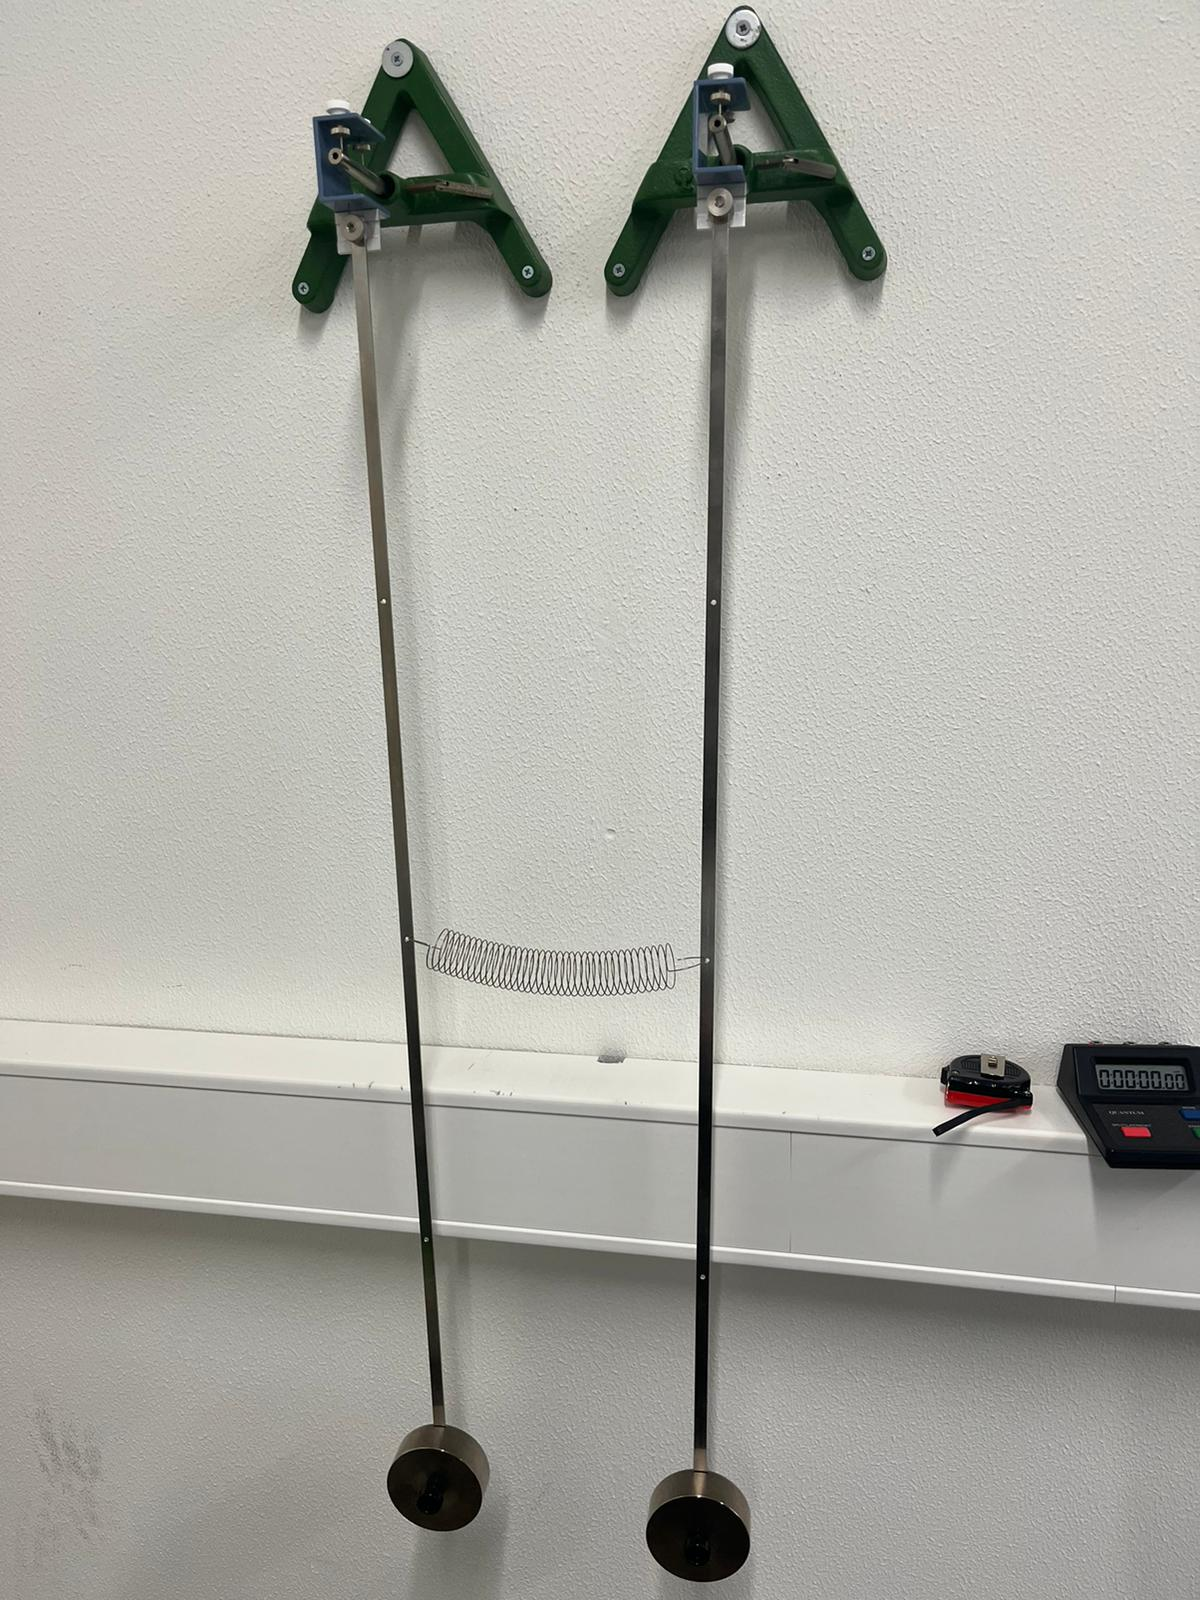
\includegraphics[height=80mm]{bilder/aufbau.jpeg}
    \caption{Die Abbildung der ganzen Versuchsmaterialien mit dem Ausgangsaufbau.\label{Abbildung2} }
\end{figure} 

\begin{flushleft}
    Für den ersten Arbeitsauftrag soll man die Schwingungsdauer für beide freischwingenden Pendel bestimmen. \\
    Dafür stellt man beide Gewichte mit dem selben Abstand zur Drehachse ein.
    Für diesen Arbeitsauftrag wird die Feder, die beide Pendel verbindet wie in Abbildung (\ref{Abbildung2}) zu sehen, nicht benötigt.
    Das erste Pendel wird jeweils um den selben Winkel wie das zweite ausgelenkt und die Schwingungsdauer gemessen.
    Eine Schwingungsdauer beträgt fünf ganze Schwingperioden. 
    Wichtg hierbei ist, dass die Schwingungsdauer nahezu gleich sein muss.
    Wenn dies nicht der Fall sein sollte ,muss ein Gewicht solange verschoben werden bis die Schwingdauer nahezu gleich ist.
    Dies wird zehn mal wiederholt für jeweils jedes Pendel.
\end{flushleft}

\begin{flushleft}
    Danach soll die Schwingdauer $ T_{+} $  für eine gleichphasige Schwingung bestimmt werden. \\
    Der Aufbau hierbei ist identisch zu dem ersten Arbeitsauftrag, jedoch wird hier eine Feder eingebaut, welche beide Pendel miteinander verbindet.
    Zusehen ist dies auch in Abbildung (\ref{Abbildung2}).
    Da die Schwingungsdauer für eine gleichphasige Schwingung bestimmt werden soll, 
    werden die Pendel im selben Abstand und Parallel zueinander ausgelenkt, verbildlicht in Abbildung (\ref{Abbildung1a}). 
    Die Schwingungsdauer beträgt ,wie im ersten Arbeitsauftrag, fünf Schwingperioden.
    Dies wird insgesamt für mindestens 10 mal wiederholt.
\end{flushleft}

\begin{flushleft}
    Als nächstes soll die Schwingungsdauer $ T_{-} $ für eine gegenphasige Schwingung bestimmt werden. \\
    Dies wird mit dem selben Aufbau wie davor ausgeführt.
    Der Unterschied bei diesem Teil ist, dass die Pendel nicht im selben Abstand parallel zueinander ausgelenkt werden,
    sondern im selben Abstand zur Ruhelage entgegengesetzt zueinander, verbildlicht in Abbildung (\ref{Abbildung1b}).
    Dies wird insgesamt für mindestens zehn male wiederholt.
\end{flushleft}

\begin{flushleft}
    Danach soll die Schwingungsdauer $ T $ und die Schwebungsdauer $ T_{s} $ für die gekoppelte Schwingung bestimmt werden. \\
    Der Versuchsaufbau ist identisch zu den zwei letzten Versuchen. 
    Bei der gekoppelten Schwingung wird zu Begin nur ein Pendel ausgelenkt und das andere bleibt in der Ruhelage.
    Beim Loslassen des ausgelenkten Pendels wird die Energie des Pendels auf das ruhende Pendel übertragen.
    Die Schwingungsdauer des ausgelenkten Pendels $ T_{ges} $ endet wenn die gesamte Energie an das vorher ruhende Pendel übergeben wurde.
    Die Schwebungsdauer $ T_{s} $ endet wenn das in Bewegung gesetzte Pendel das erste Mal wieder ruht.
    Dies wird insgesamt für mindestens zehn male wiederholt.
\end{flushleft}

\begin{flushleft}
    Alle Durchführungen werden wiederholt mit einem anderen Abstand zur Drehachse.
    Der Abstand im ersten Durchgang beträgt $ 0,78\,\unit{\meter} $ und im zweiten Durchgang $ 0,99\,\unit{\meter} $
\end{flushleft}